\documentclass{beamer}
\usetheme{Hannover}
\usepackage{polski}
\usepackage{customcolortheme}
\usepackage{tikz}
\usepackage{listings}
\usepackage{booktabs}

\title{
\includegraphics[trim={1cm 1cm 1cm 1cm}, clip, width=0.3\textwidth]{logo_project}\\[1em] finansowy-kompas.com.pl}
\subtitle{Rozpocznij analizę\\ swojej przyszłości! \\[-2em]}
%\author{Kwarta}
\institute{
\includegraphics[trim={1.1cm 1.1cm 1.1cm 1.1cm}, clip, width=0.07\textwidth]{long_shadow}\\ Kwarta}
\date{\today}

\begin{document}

\frame{\titlepage}

\begin{frame}
\frametitle{Plan prezentacji}
\tableofcontents
\end{frame}


% ============================================
\section{Opis problemu}
% ============================================

\begin{frame}
\frametitle{Stan kalkulatorów emerytalnych na 2025 rok}

\includegraphics[width=.8\textwidth]{img/zus_calculator_01}
\end{frame}

\begin{frame}
\frametitle{Stan kalkulatorów emerytalnych na 2025 rok}
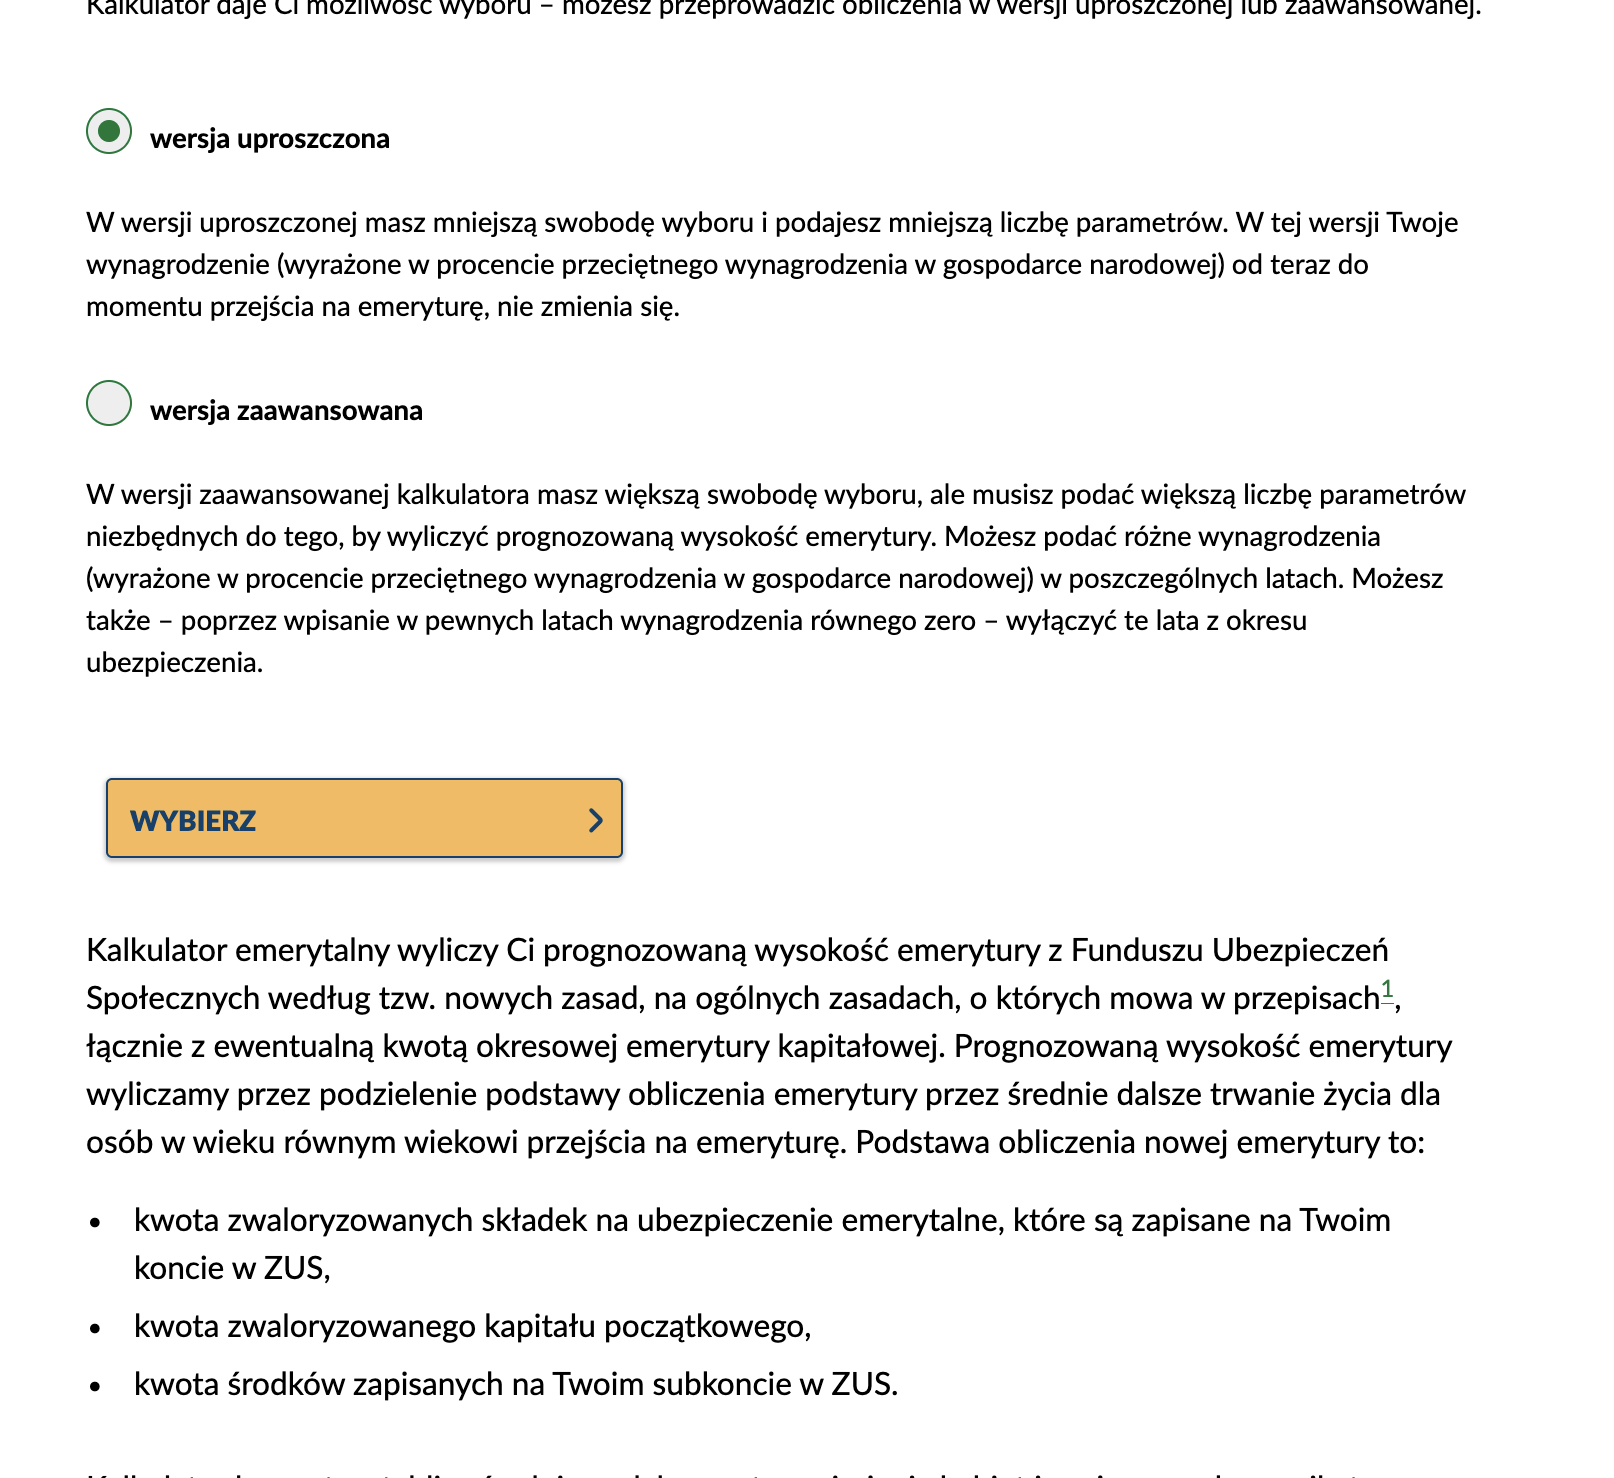
\includegraphics[width=.8\textwidth]{img/zus_calculator_02}
\end{frame}

\begin{frame}
\frametitle{Stan kalkulatorów emerytalnych na 2025 rok}
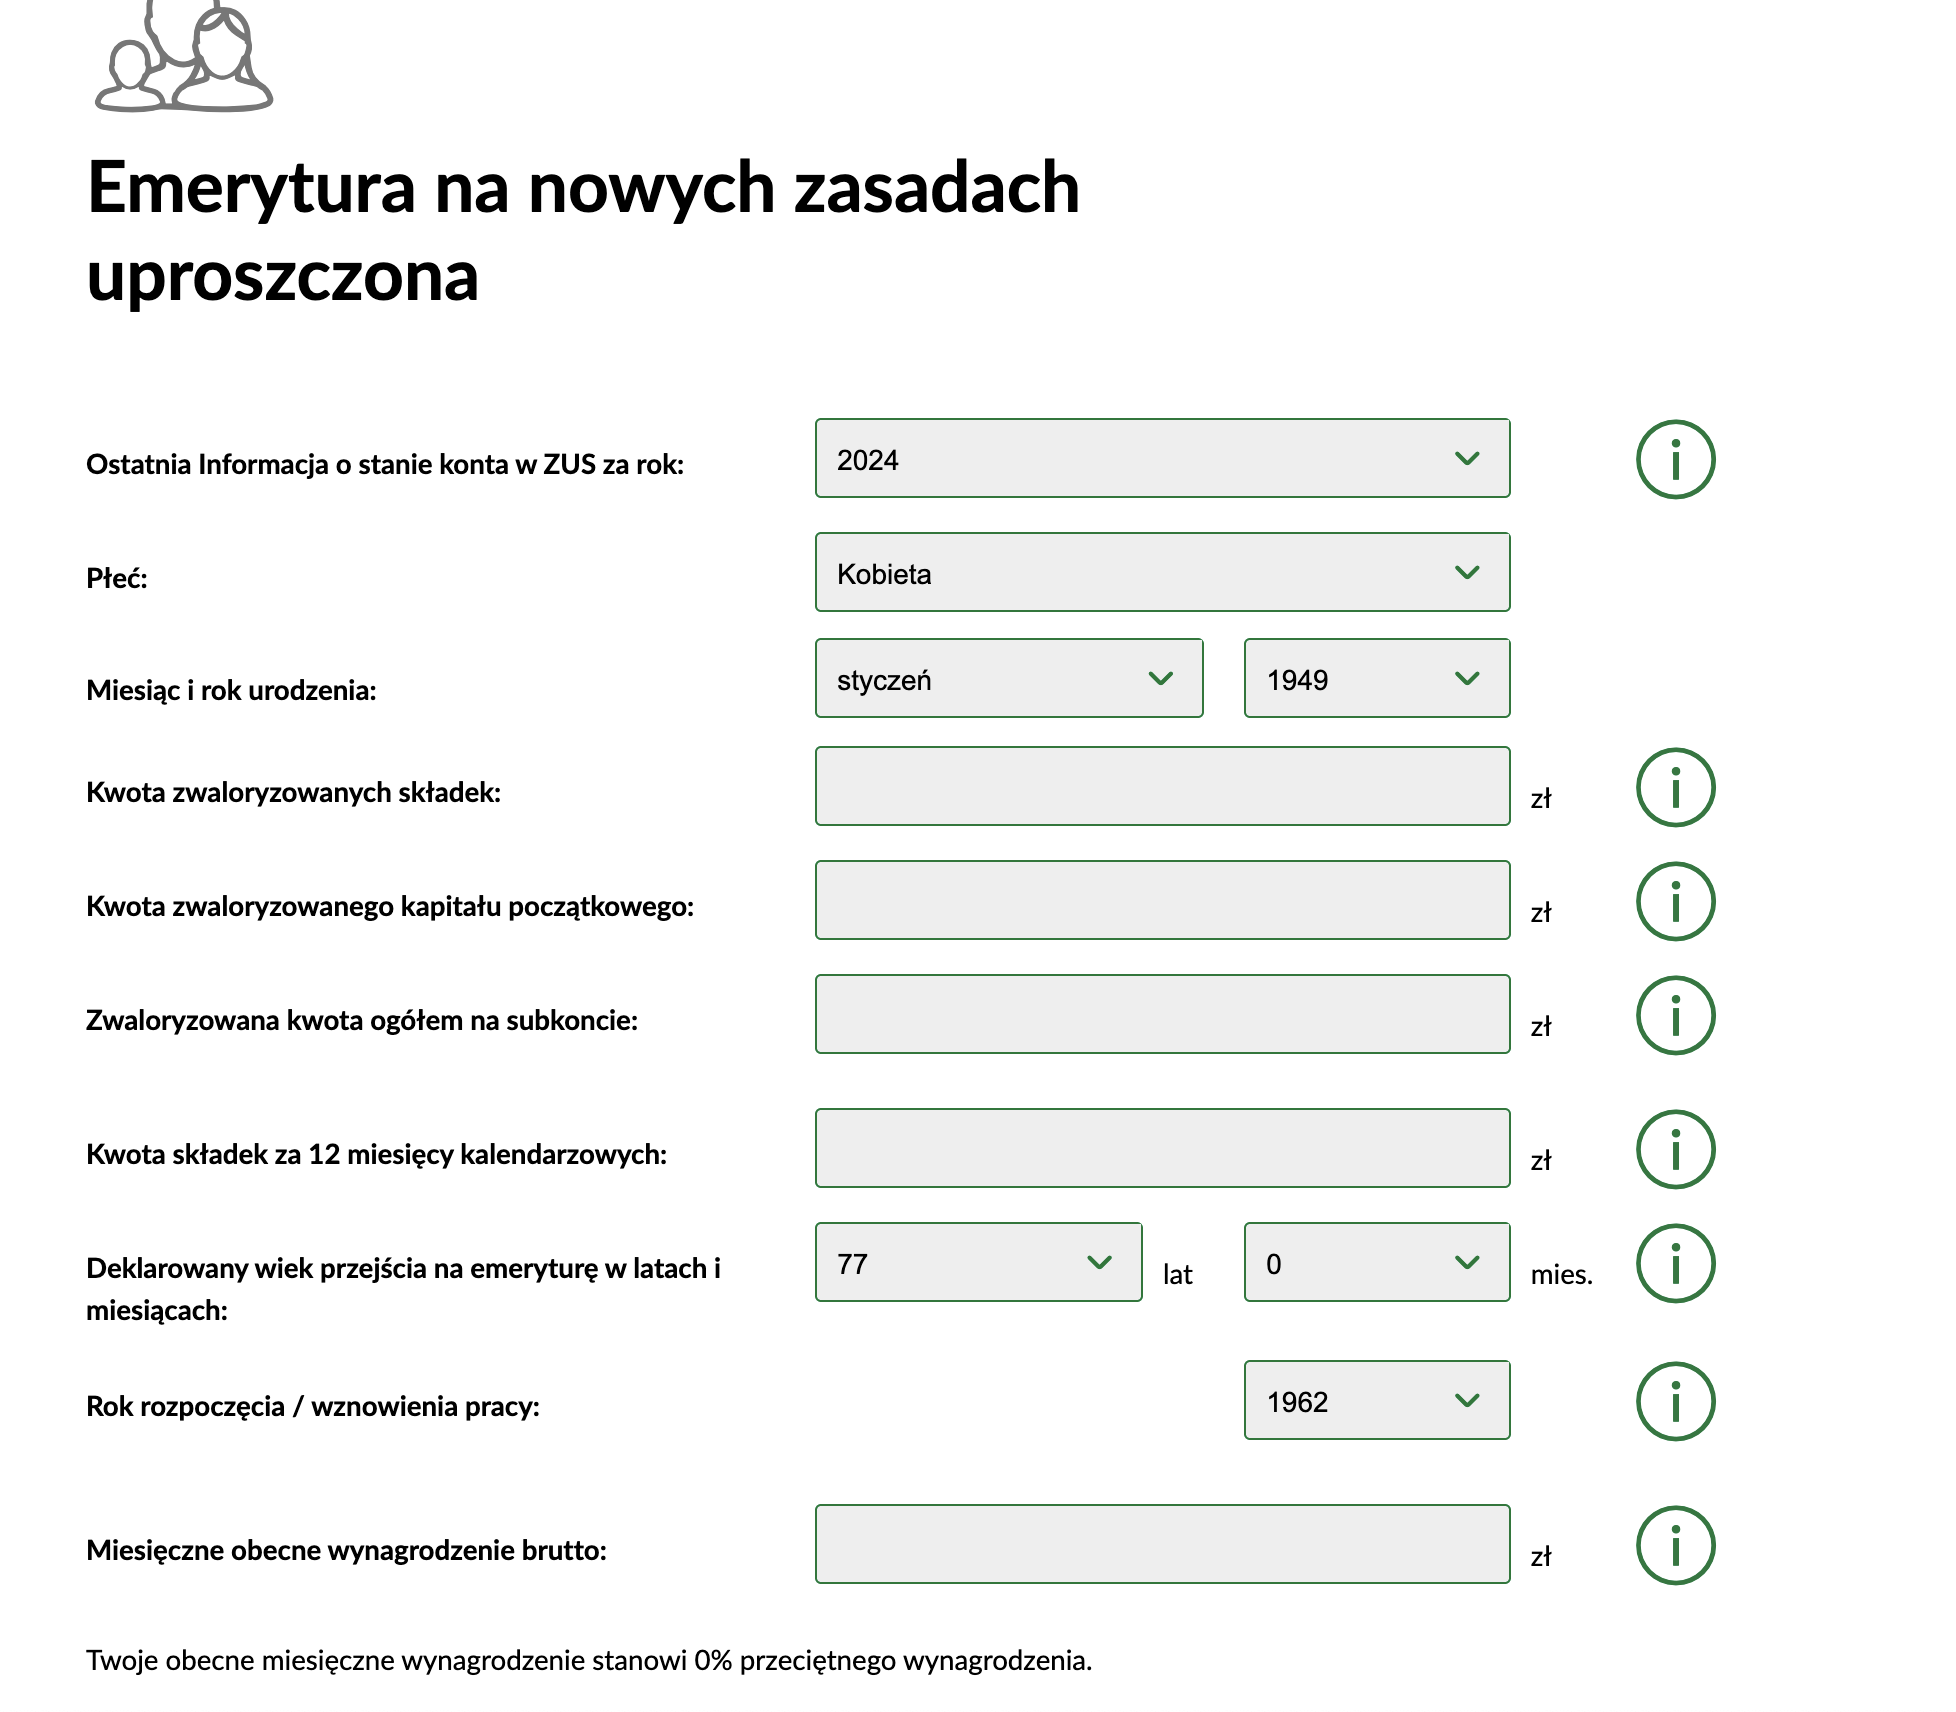
\includegraphics[width=.8\textwidth]{img/zus_calculator_03}
\end{frame}

% ============================================
\section{Konkretyzacja wyzwań}
% ============================================

\begin{frame}
\textbf{Plątanina nieznanych pojęć:}
    \pause
\begin{itemize}
    \item nie wiadomo, od czego zacząć
    \pause
    \item wyjaśnienia \emph{ignotum per ignotum}, często zapętlone
    \pause
    \item każdy indywidualny przypadek jest inny --- nie ma jednego wzorca, uniwersalnego wzoru
\end{itemize}
\end{frame}

\begin{frame}
\frametitle{Wybrane technologie i metody analizy danych}
\textbf{Wykorzystujemy nowoczesne narzędzia, które umożliwiają nam zaradzeniu każdemu z tych wyzwań!}
    \pause
\begin{itemize}
    \item Zebrane dane historyczne (inflacja, wskaźnik PKB itp.)
    \pause
    \item Modele uczenia maszynowego przewidujące i klasyfikujące przyrost wynagrodzenia wynikający z progresji kariery
    \pause
    \item Modele językowe LLM wspomagane wyszukiwaniem zasobów sieciowych RAG
\end{itemize}
\end{frame}

% ============================================
\section{Modele i regresje}
% ============================================

\begin{frame}
    \frametitle{Model ML}
    \begin{equation}
    k(x) = 1 + \alpha (1 - e^{-\beta x})
    \end{equation}
    \pause
    $x$ --- lata doświadczenia w zawodzie
    \pause
    $\textrm{pensja} \pause = \textrm{pensja juniora} \pause \cdot k(x)$
\end{frame}

\begin{frame}[plain]
    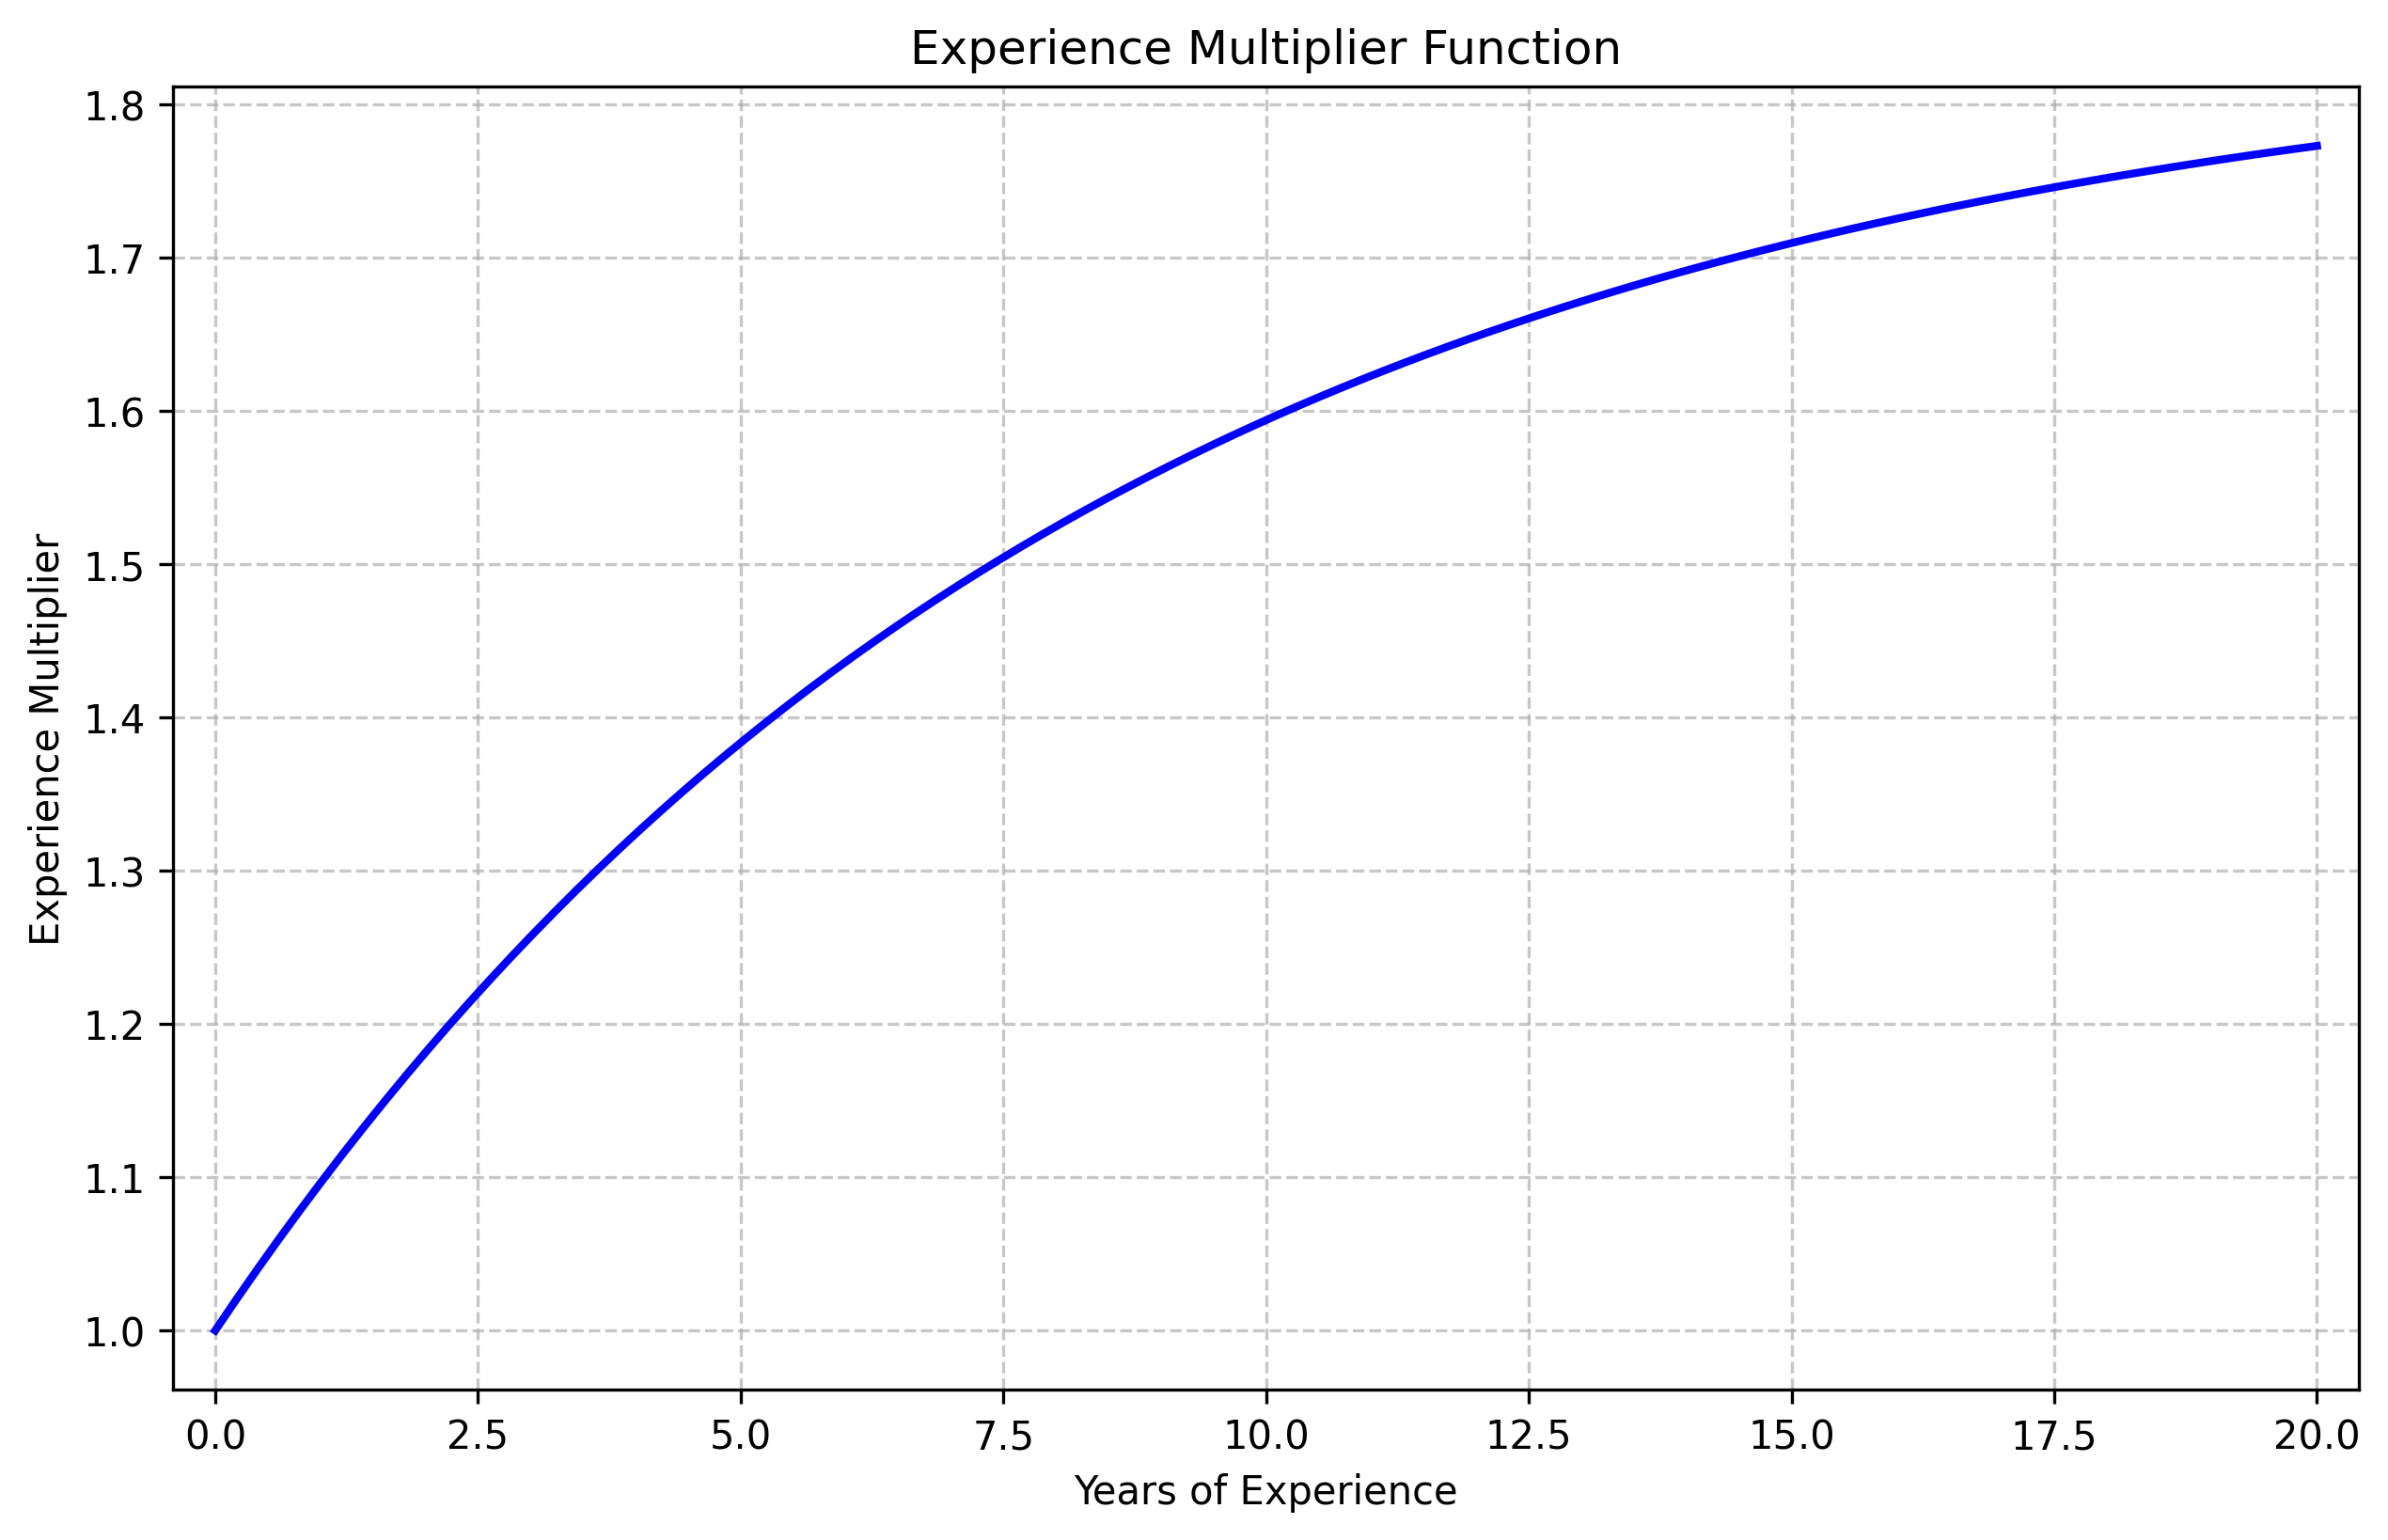
\includegraphics[width=.8\textwidth]{img/experience_multiplier}
\end{frame}

\begin{frame}
\centering
\begin{tabular}{cc}
    \pause
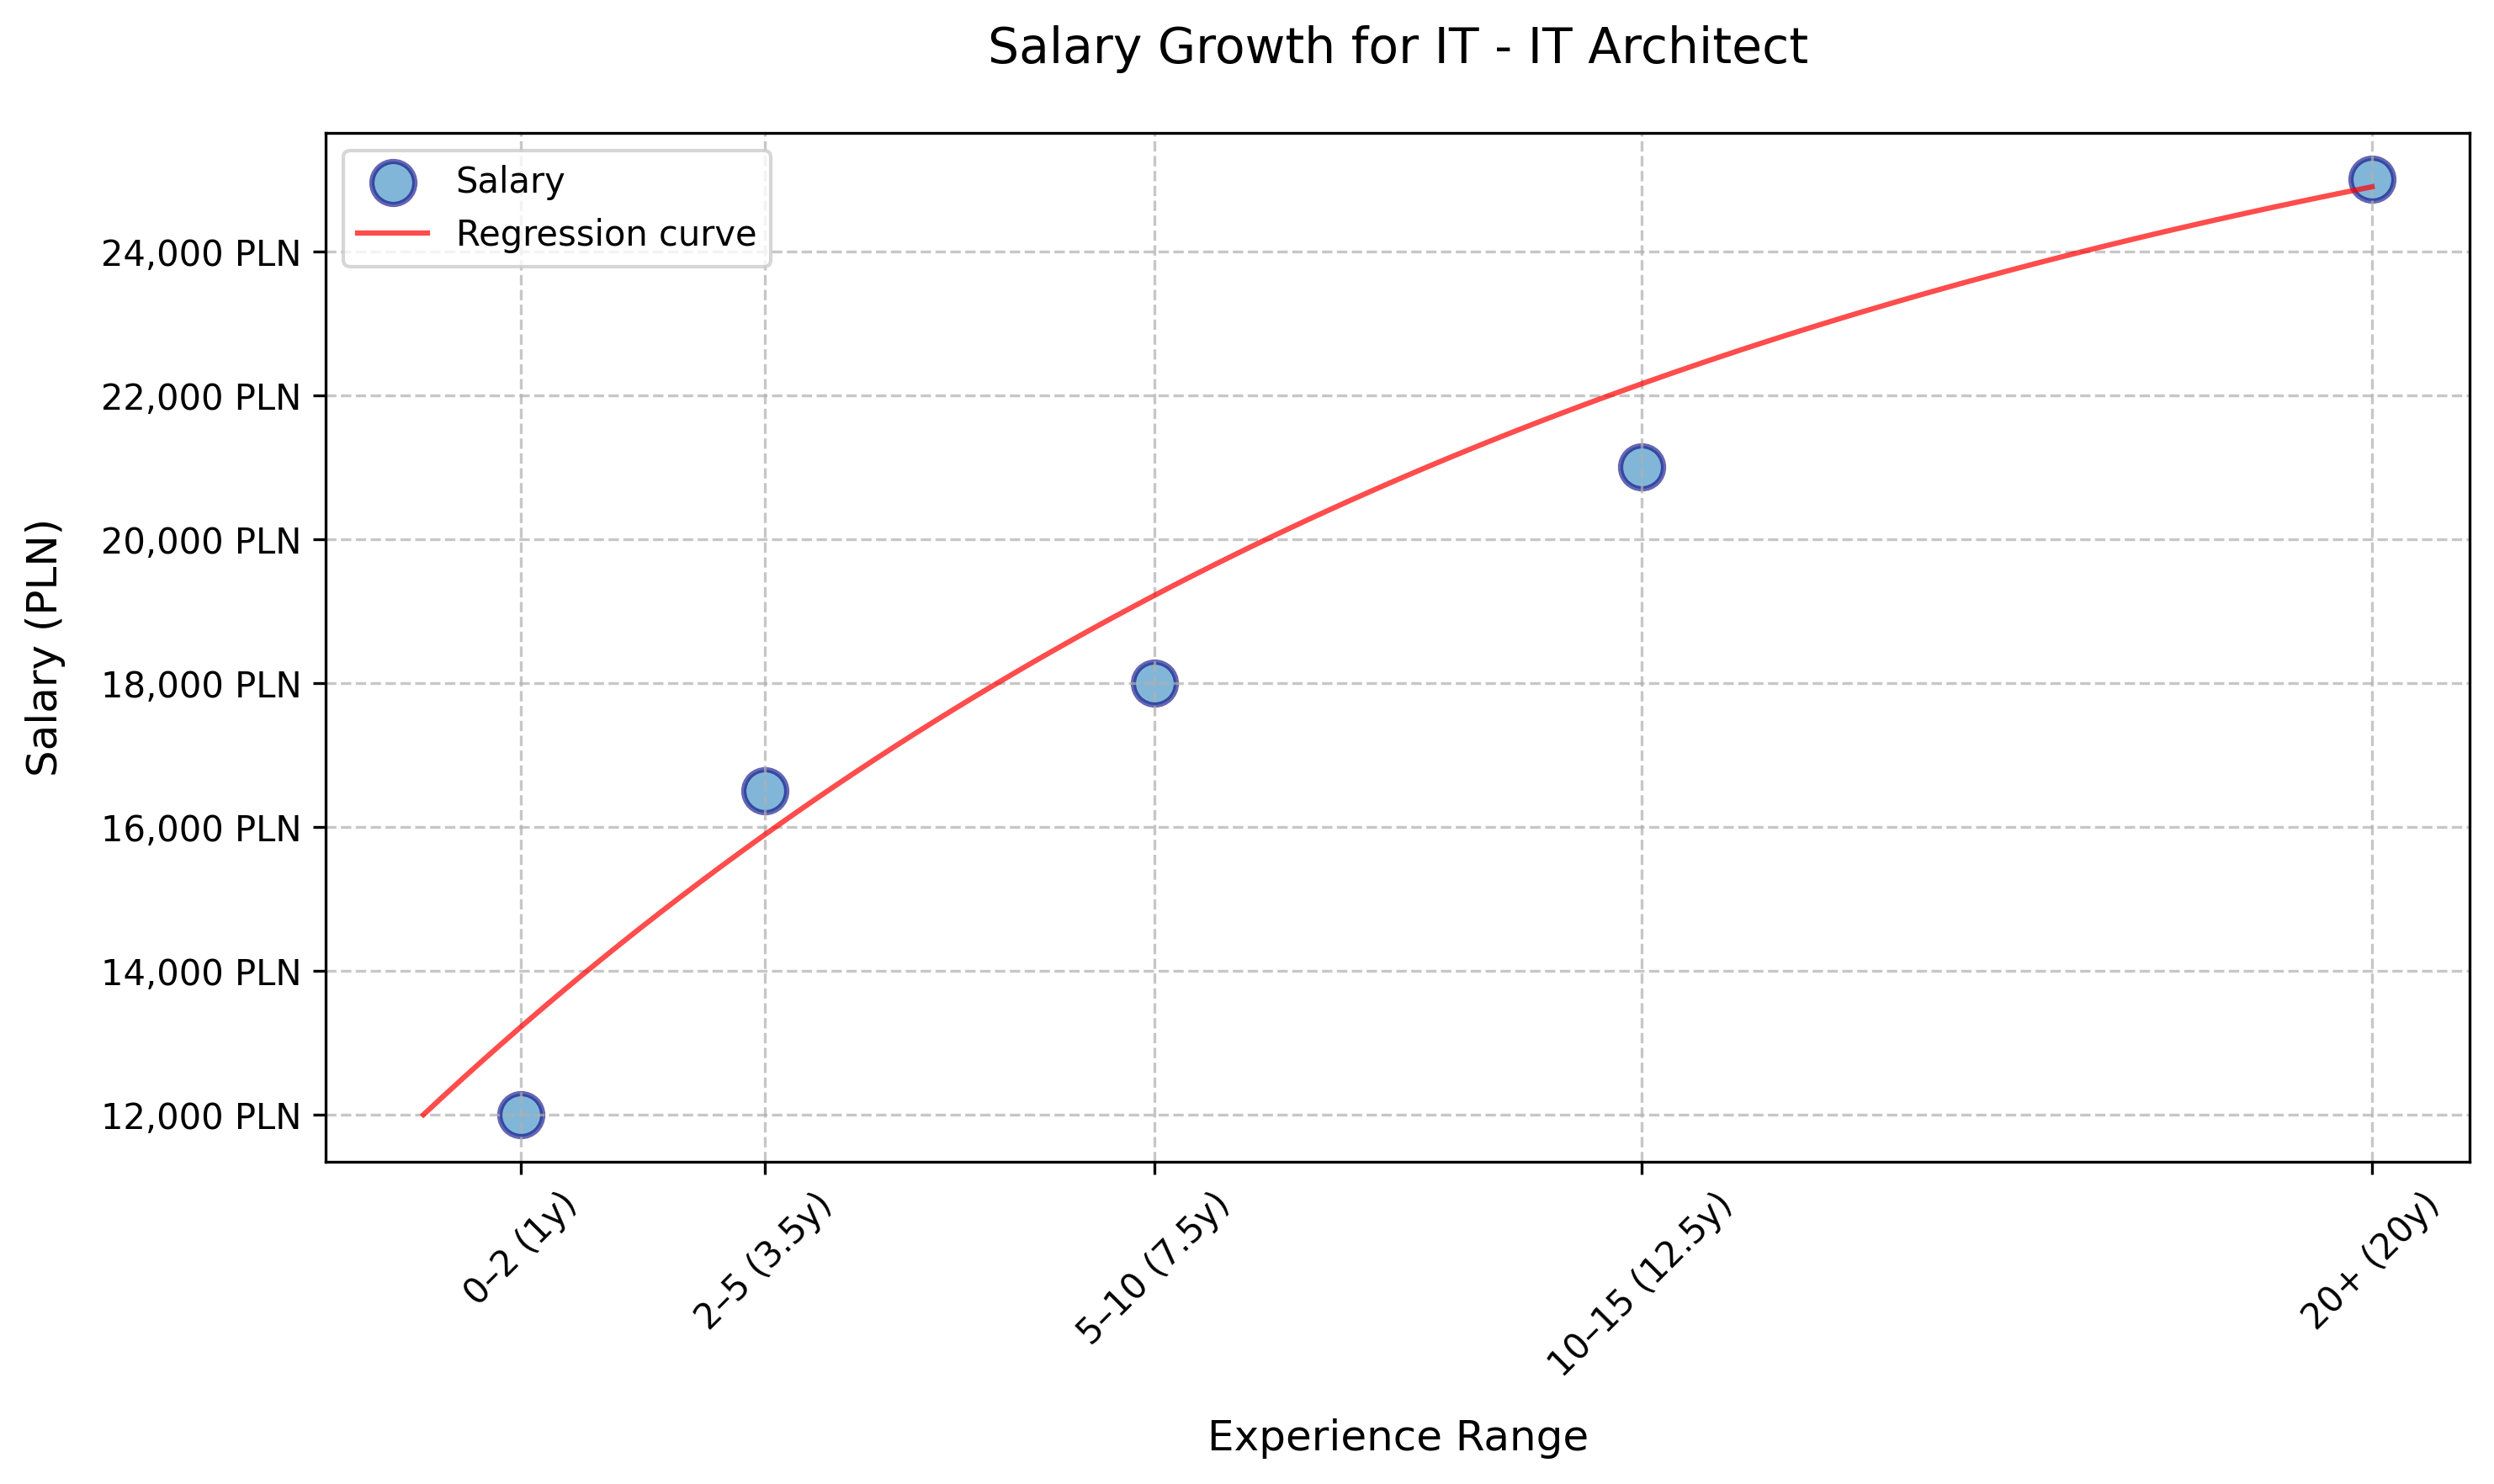
\includegraphics[width=0.45\linewidth]{img/salary_progression2} &
    \pause
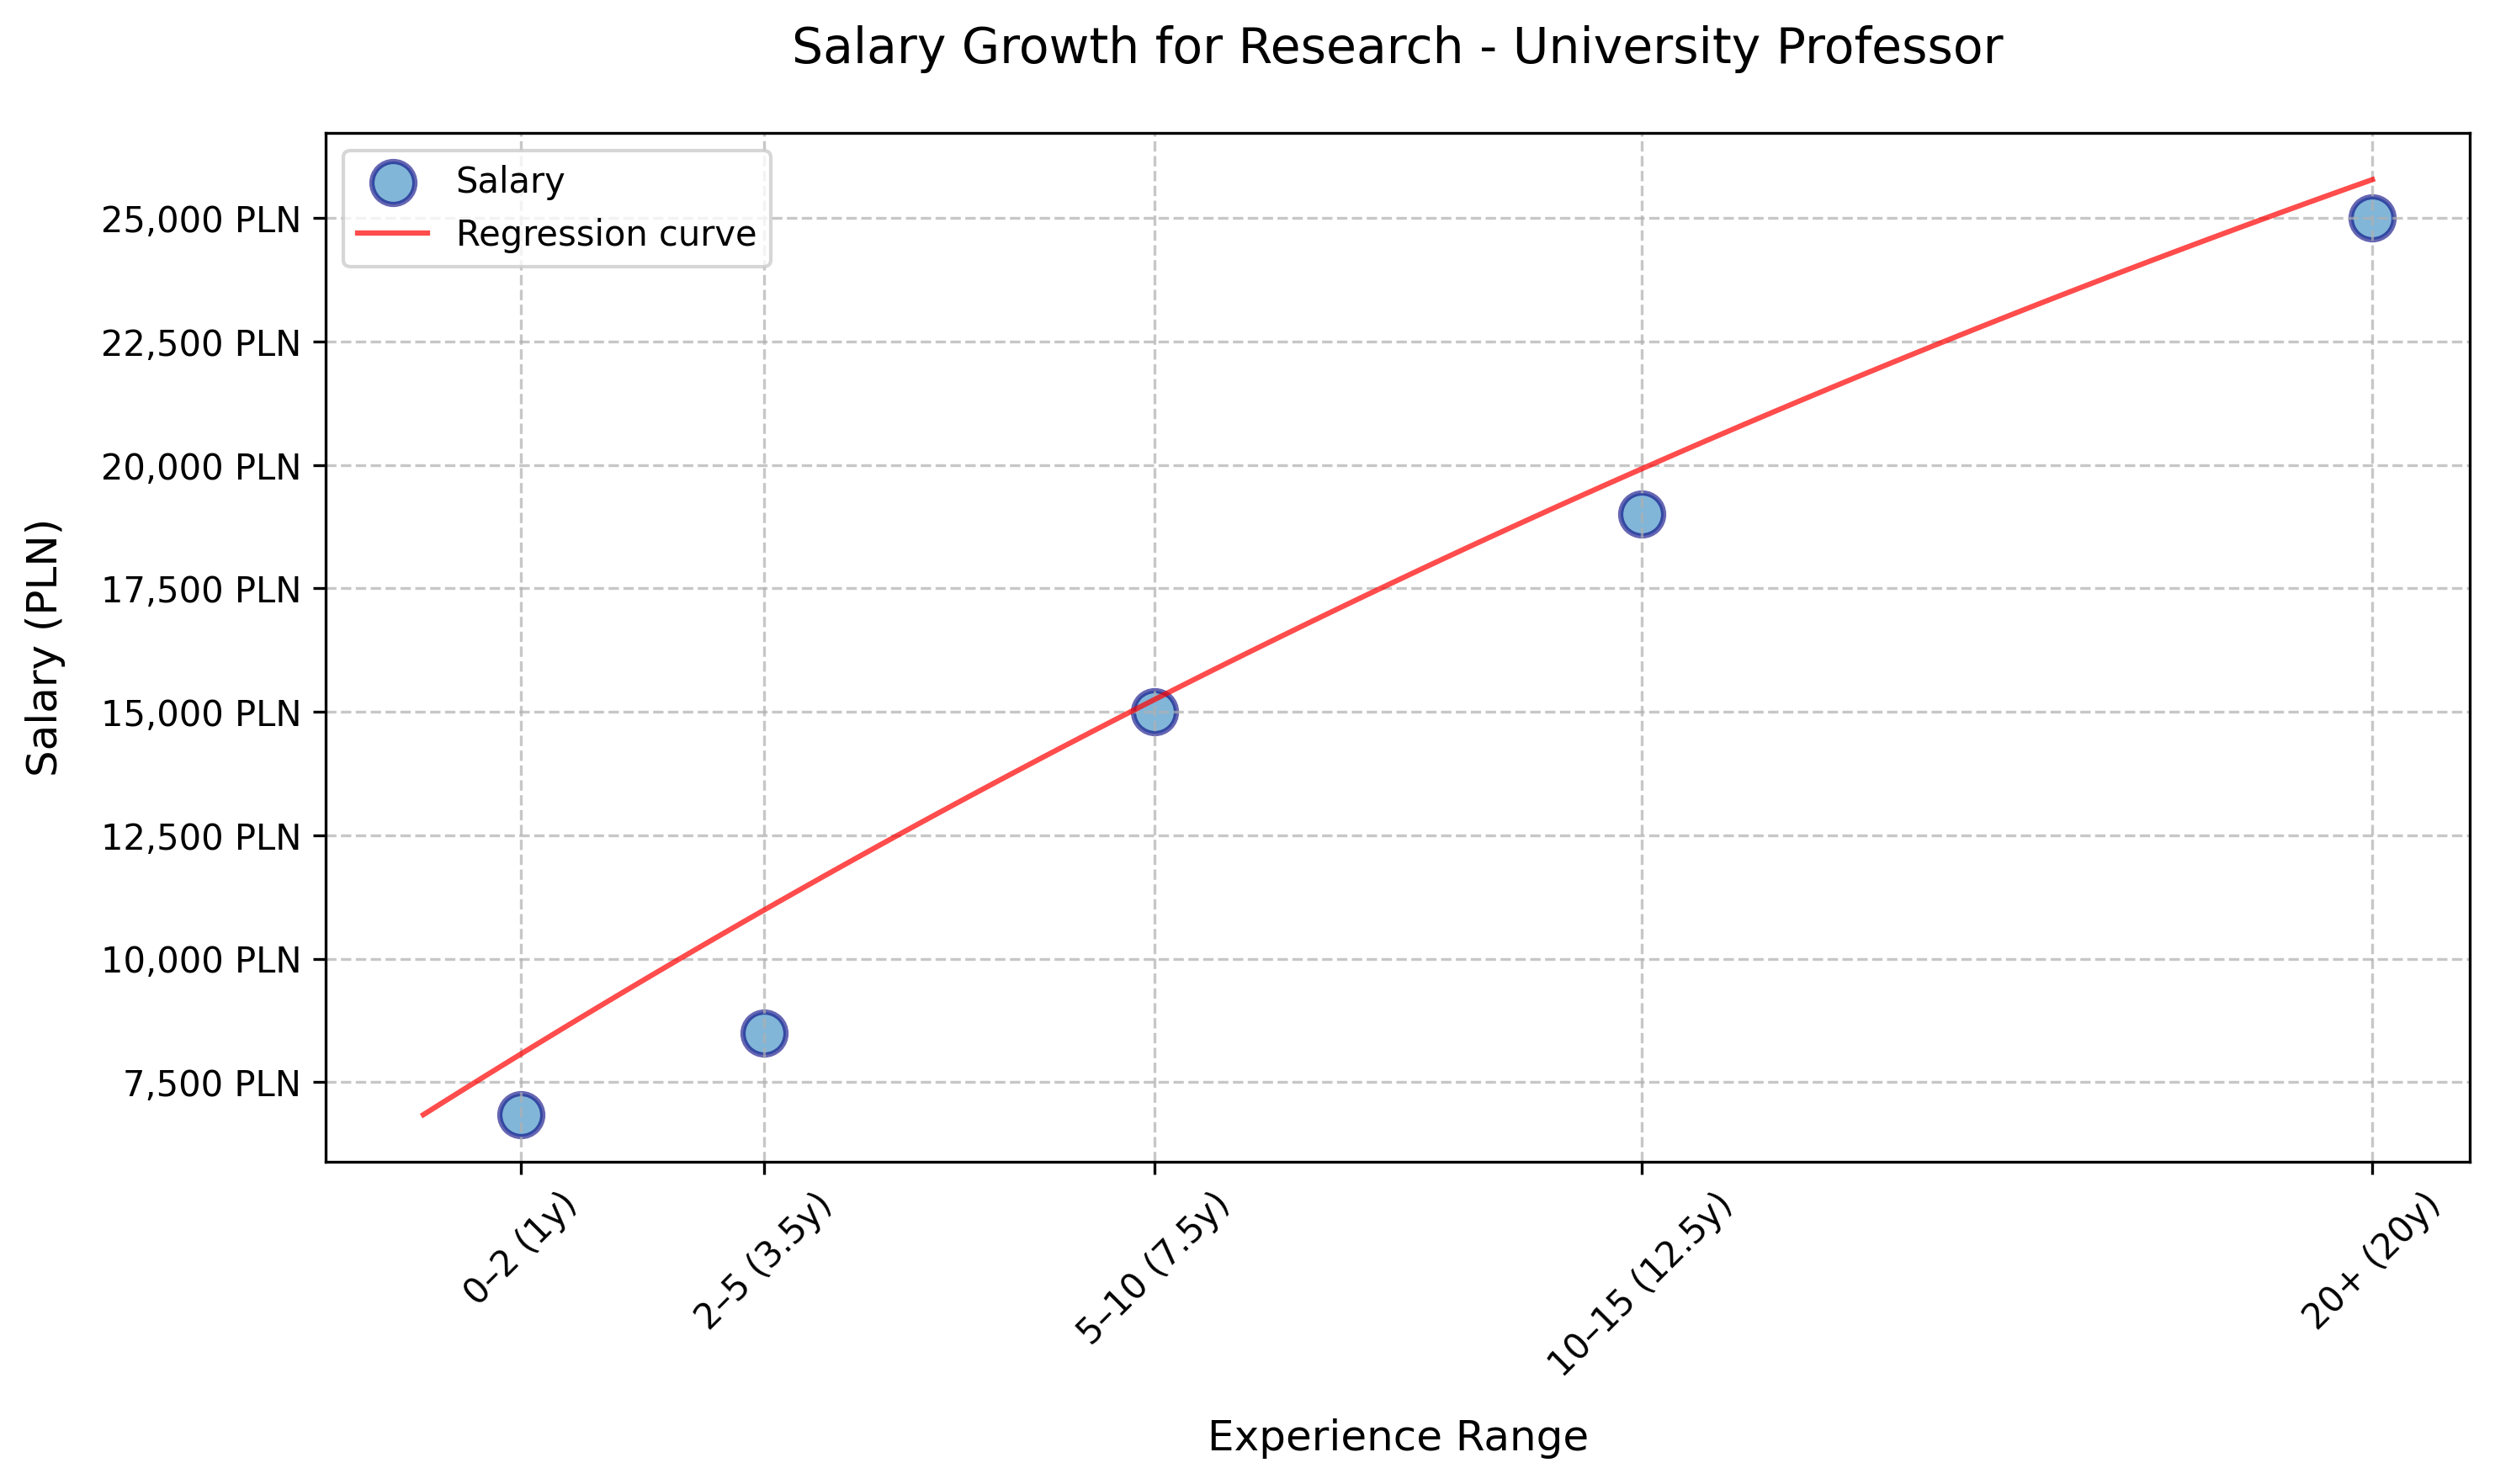
\includegraphics[width=0.45\linewidth]{img/salary_progression4} \\
    \pause
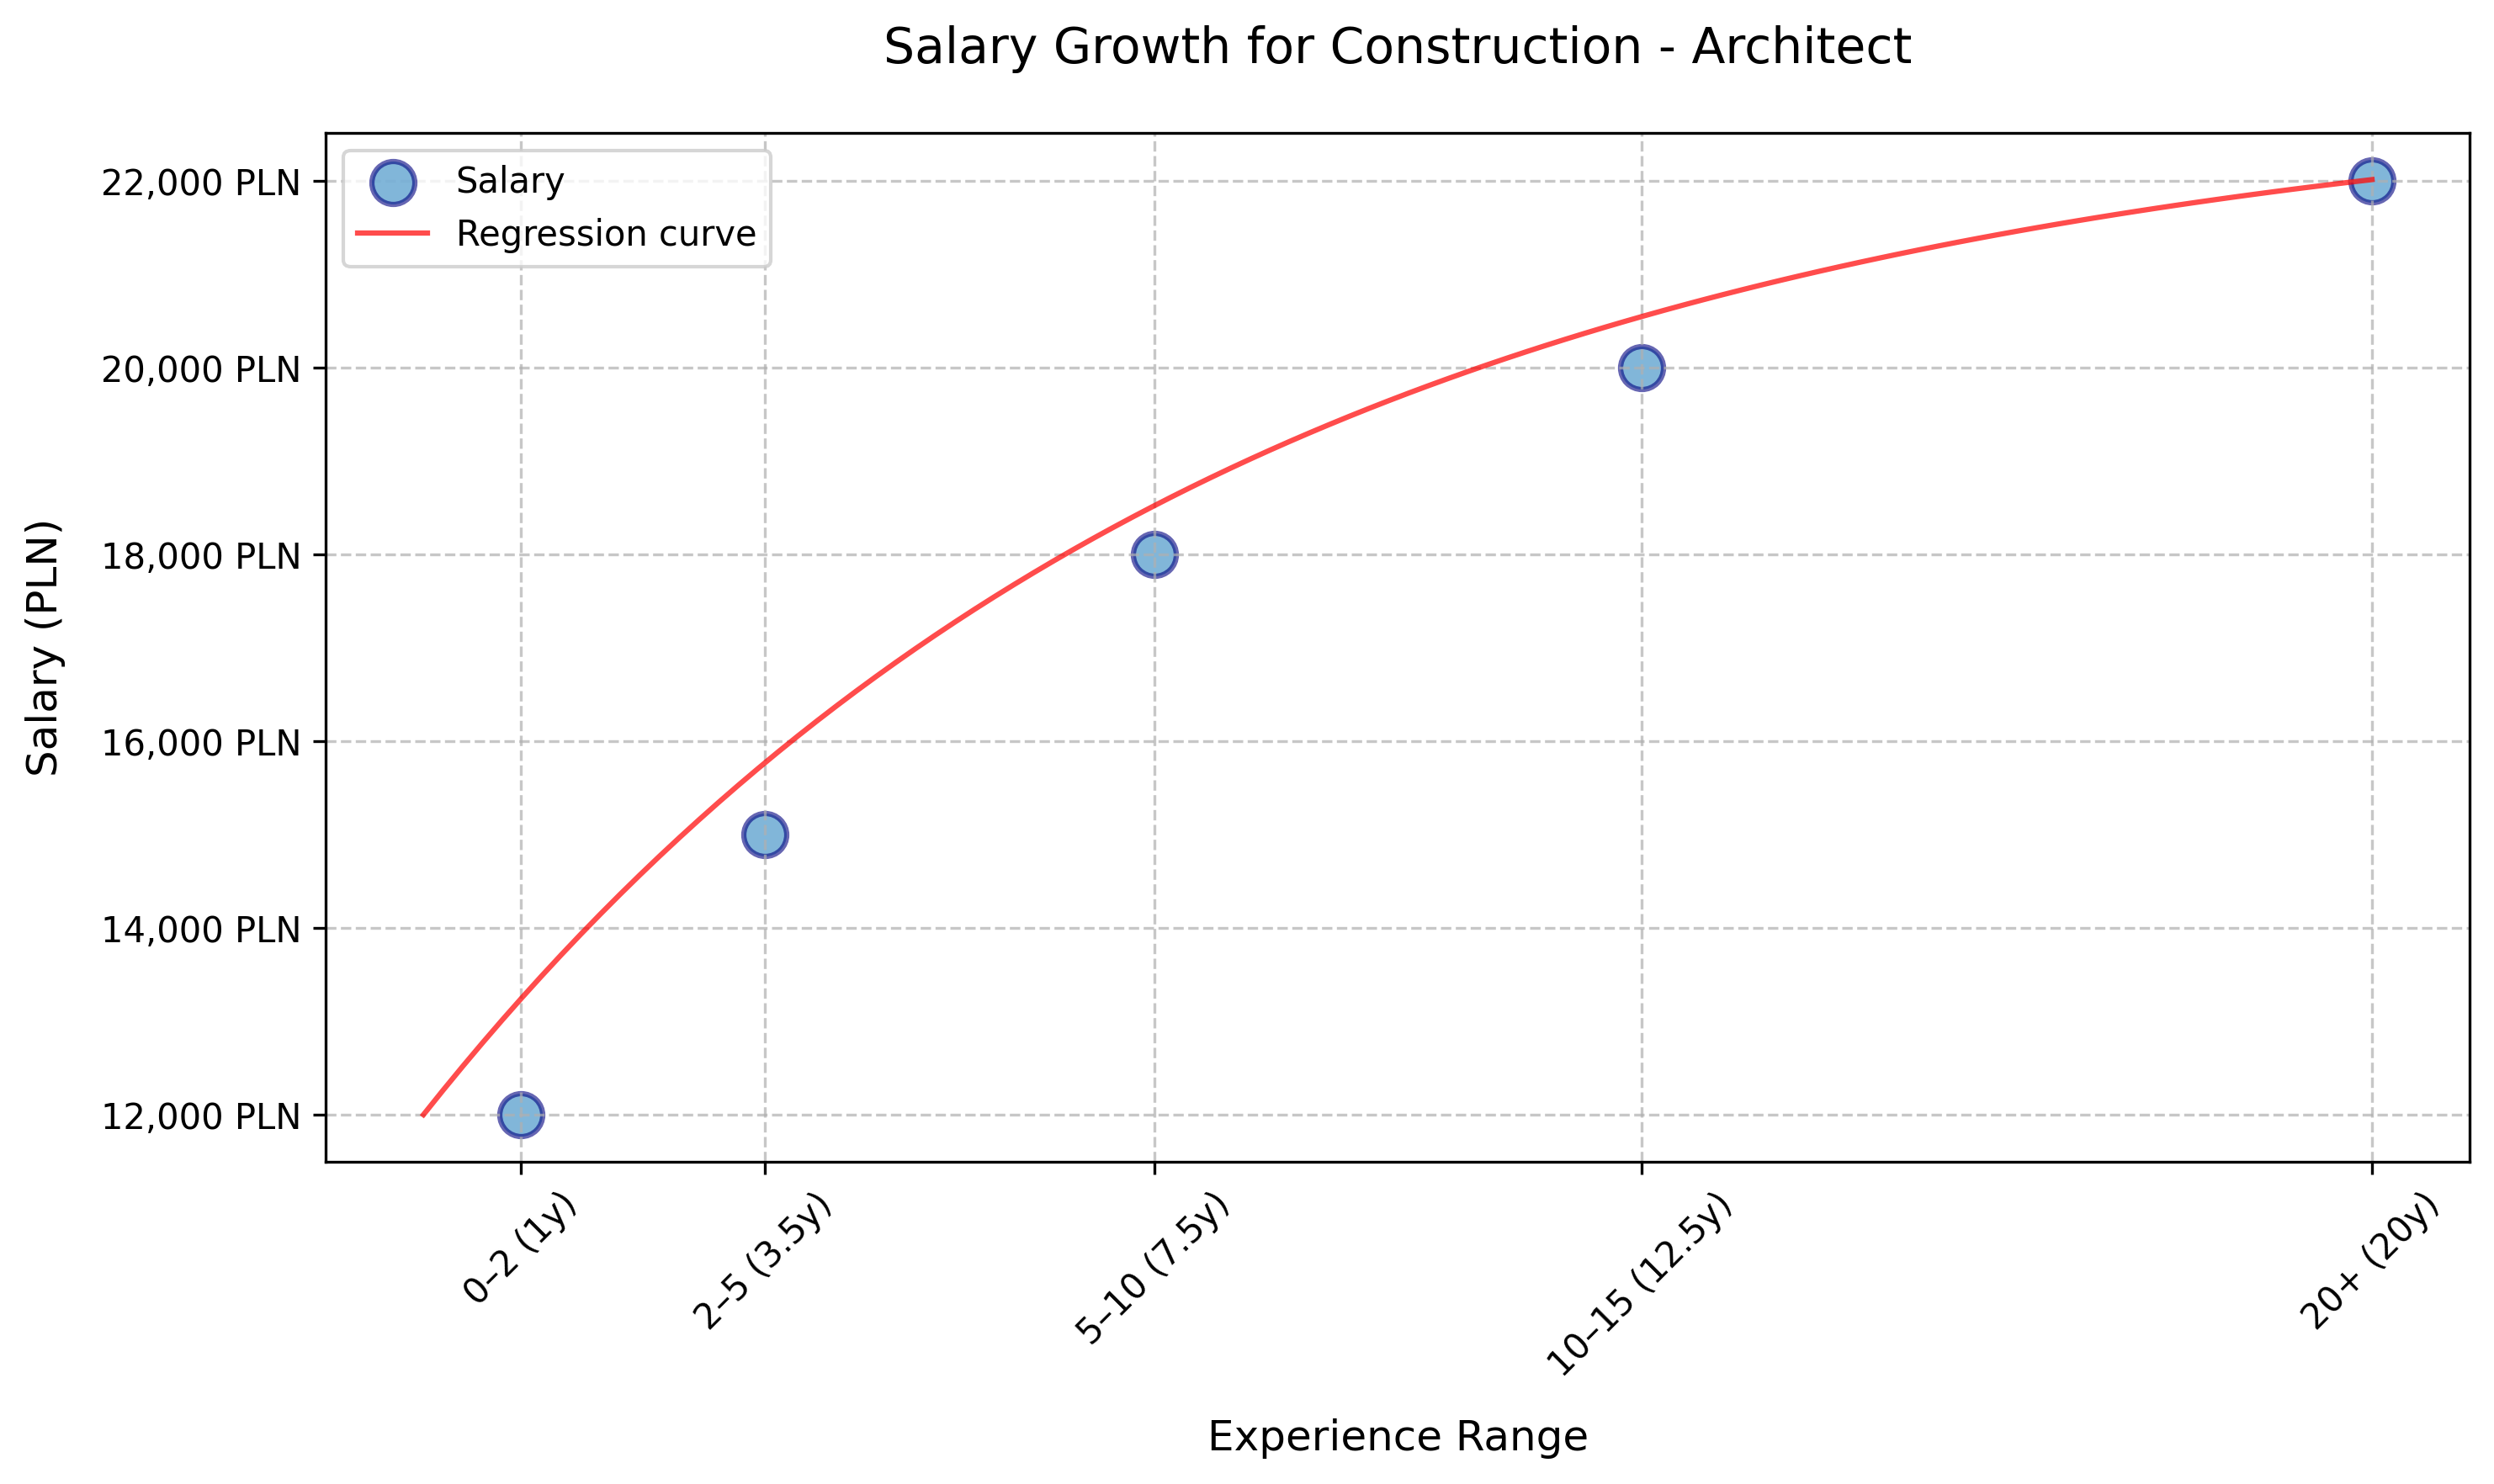
\includegraphics[width=0.45\linewidth]{img/salary_progression6} &
    \pause
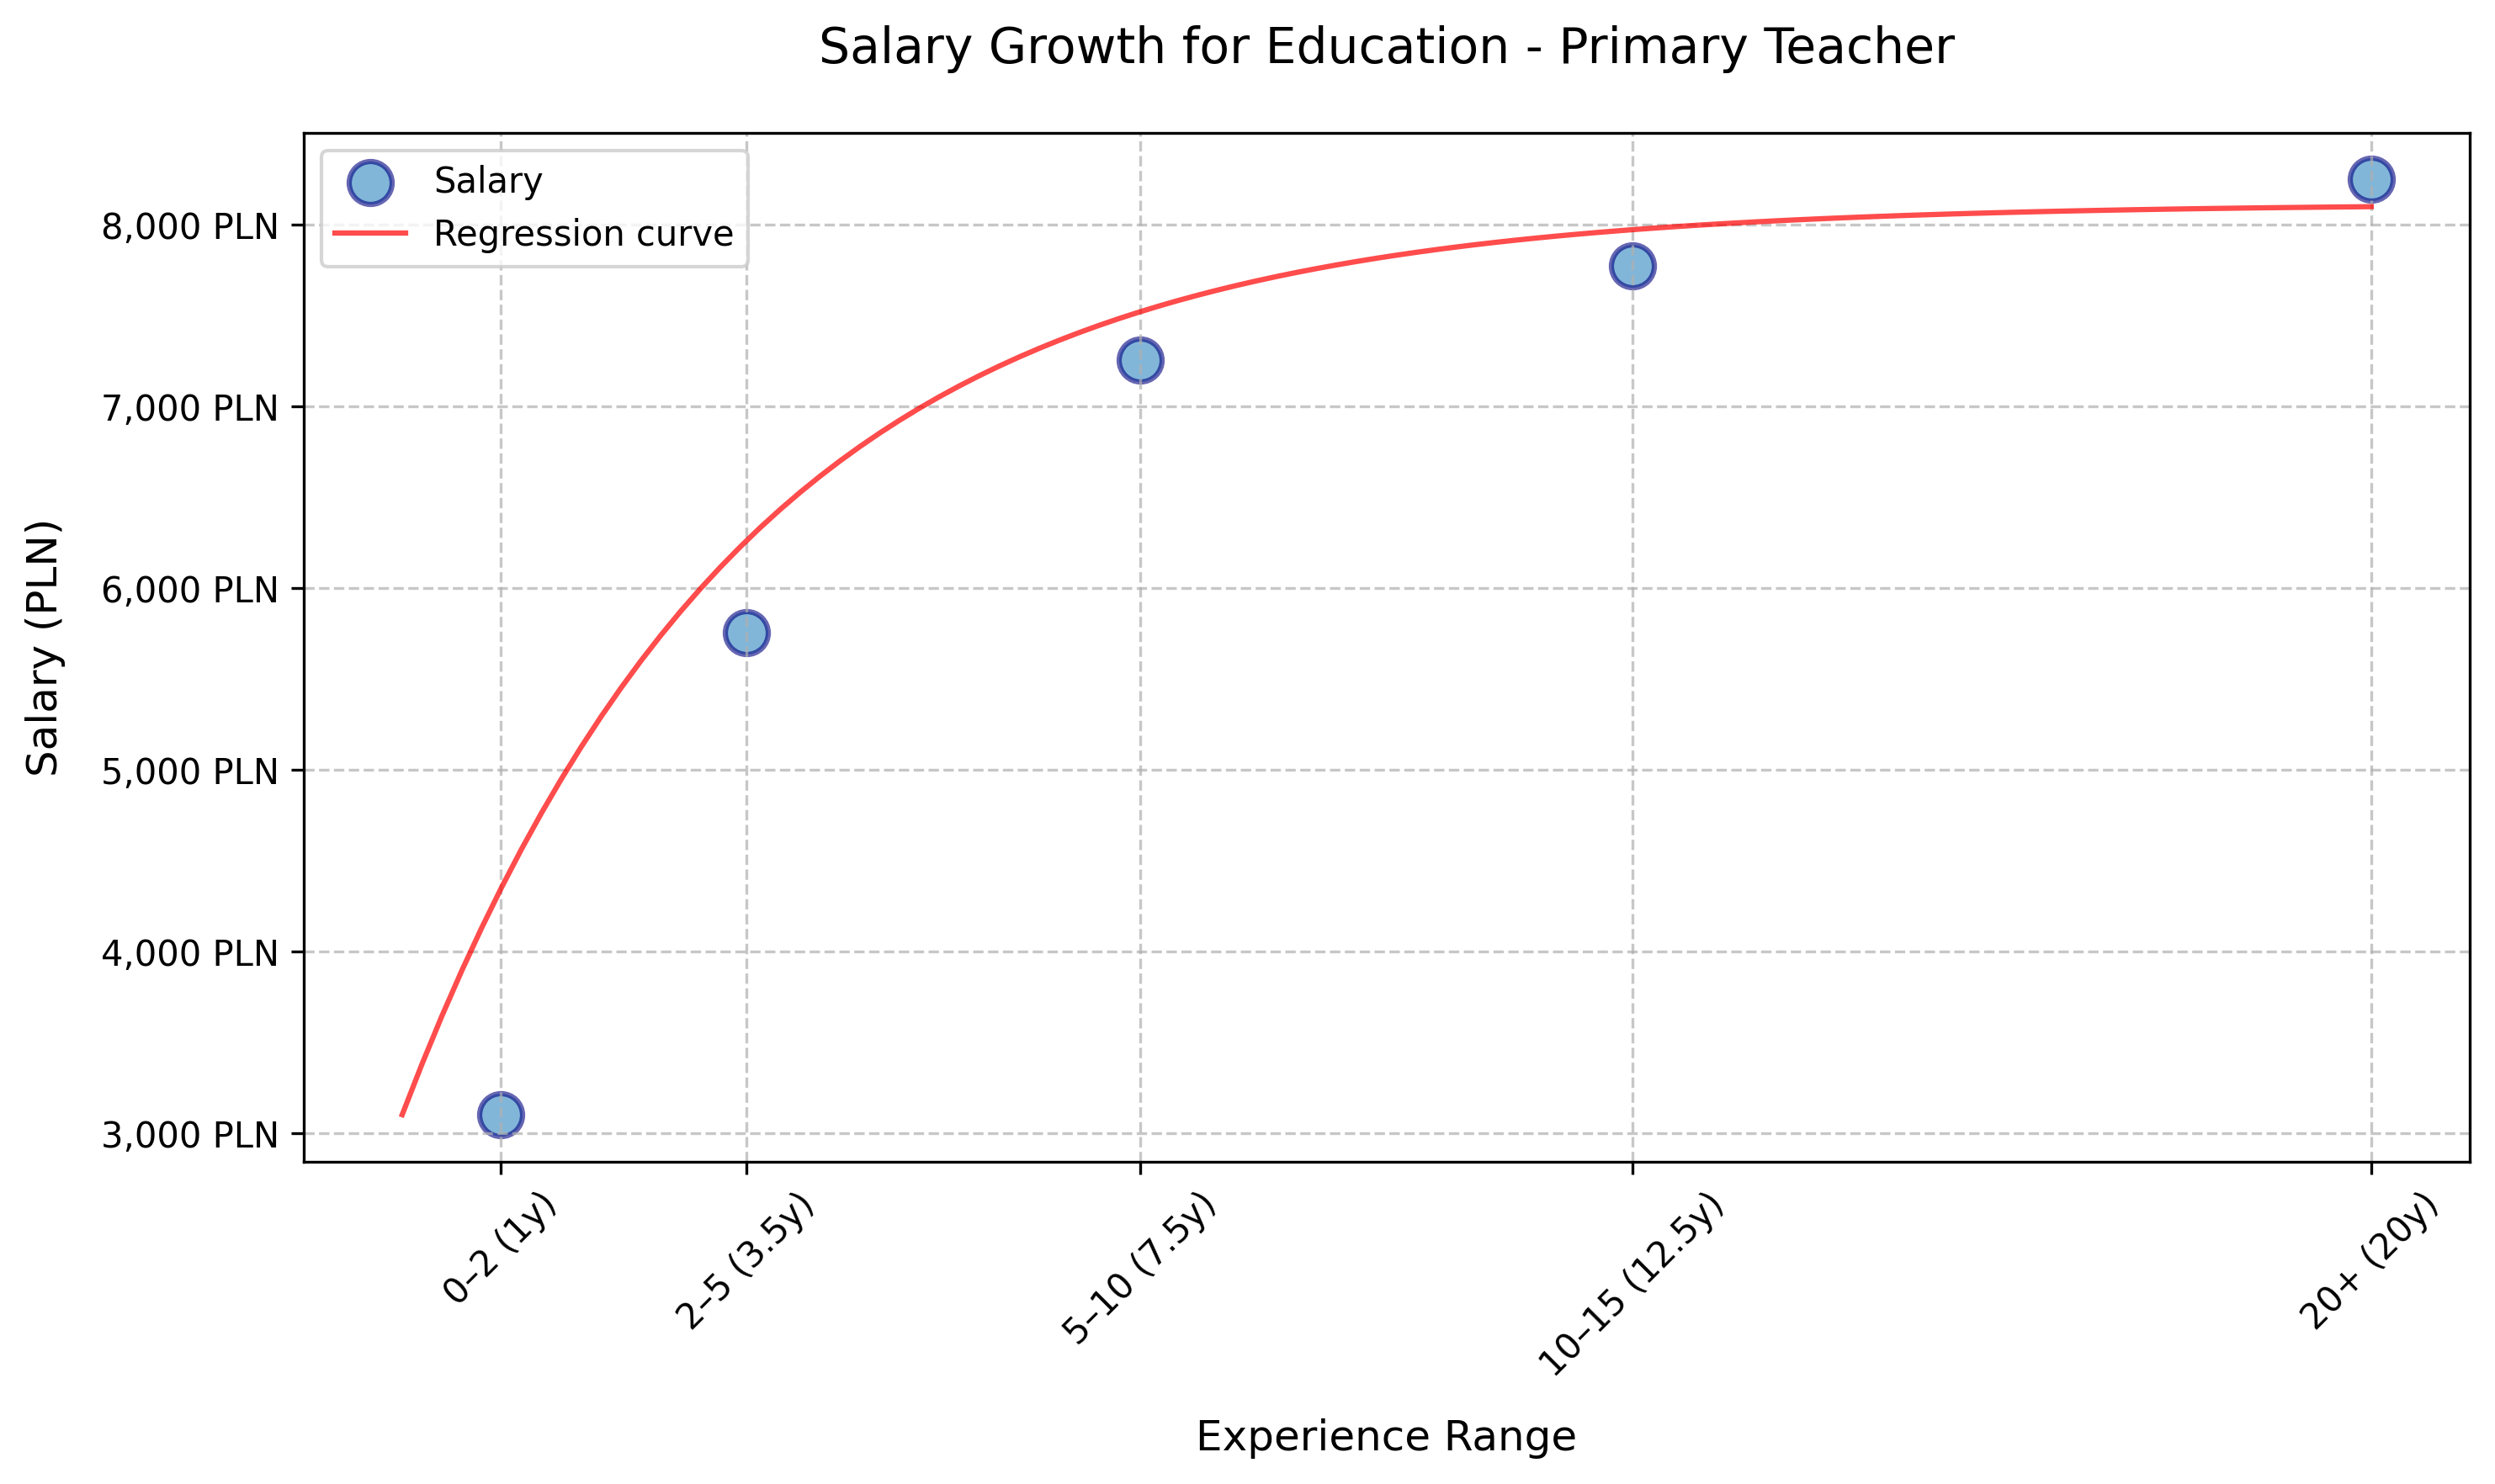
\includegraphics[width=0.45\linewidth]{img/salary_progression7}
\end{tabular}
\end{frame}

\begin{frame}
\frametitle{LLM i RAG}
    \textbf{Wykorzystując API Gemini możemy dokonać klasyfikacji dowolnego zawodu do jendego,
        z uprzednio wytrenowanych modeli.}
    \\
    \pause
    \brand{Przy użyciu technologii RAG (\emph{Retrieval-Augmented Generation})
    znajdujemy aktualną stawkę świeżo zatrudnionego juniora danej branży}
    \\
    \pause
    \highlight{Dokładając model czynników makroekonomicznych takich, jak inflacja czy przyrost PKB
    jesteśmy w stanie sensownie oszacować całą finansową historię użytkownika - zarówno przeszłą jak i przyszłą!}
\end{frame}

% ============================================
\section{Rezultat}
% ============================================

\begin{frame}
    \frametitle{Użycie modeli w aplikacji}
    \textbf{Nasz model pozwala przeistoczyć prosty kalkulator składek emerytalnych
    w inteligentnego przewodnika po świecie zależności finansowych, który samodzieline sugeruje
    szereg parametrów!}
    \\
    \pause
    \brand{Normalnie zebranie tego typu danych wymagałoby przegrzebania }
\end{frame}

\begin{frame}
\textbf{Ordered Lists:}
\begin{enumerate}
    \item Numbers also use primary color
    \item Consistent with brand identity
    \item \highlight{Highlights} use secondary color
\end{enumerate}

\muted{This is muted text for less important information.}
\end{frame}

\begin{frame}
\frametitle{Color Palette Demo}
\begin{itemize}
    \item This uses our \highlight{custom color system}
    \item Primary color for structure elements
    \item \muted{Muted text for secondary information}
    \item Consistent with design tokens approach
\end{itemize}
\end{frame}

\begin{frame}
\frametitle{Block Examples}

\begin{block}{Standard Block}
Uses primary color
\end{block}

\begin{alertblock}{Alert Block}
Uses error/warning color
\end{alertblock}

\begin{exampleblock}{Example Block}
Uses success color
\end{exampleblock}

\end{frame}

\begin{frame}
\frametitle{Text Formatting}

\textbf{Bold text} and \textit{italic text} \\
\alert{Alert text uses error color} \\
\structure{Structure color is our primary} \\

\vspace{1em}
Custom commands:
\begin{itemize}
    \item \brand{Brand color} for emphasis
    \item \highlight{Highlight} for attention
    \item \muted{Muted} for secondary info
\end{itemize}
\end{frame}

% ============================================
\section{Blocks and Boxes}
% ============================================

\begin{frame}
\frametitle{Block Types}

\begin{block}{Standard Block}
Uses primary color background for title. Perfect for definitions, theorems, or key concepts.
\end{block}

\begin{alertblock}{Alert Block}
Uses error color to draw attention to warnings or important notes.
\end{alertblock}

\begin{exampleblock}{Example Block}
Uses success color for examples, solutions, or positive outcomes.
\end{exampleblock}

\end{frame}

% ============================================
\begin{frame}
\frametitle{Columns Layout}

\begin{columns}[T]
\column{0.5\textwidth}
\begin{block}{Left Column}
    \begin{itemize}
        \item Point one
        \item Point two
    \end{itemize}
\end{block}

\column{0.5\textwidth}
\begin{exampleblock}{Right Column}
    \begin{itemize}
        \item Example A
        \item Example B
    \end{itemize}
\end{exampleblock}
\end{columns}

\vspace{1em}
Great for comparisons or side-by-side content!
\end{frame}

% ============================================
\section{Advanced Features}
% ============================================

\begin{frame}
\frametitle{Overlays and Animations}
\framesubtitle{Progressive disclosure}

\begin{itemize}
    \item<1-> First item appears immediately
    \item<2-> Second item appears on click
    \item<3-> Third item appears next
    \item<4-> \highlight{Highlighted} items can appear last
\end{itemize}

\vspace{1em}

\only<2>{This text only appears on slide 2}
\only<3->{This text appears from slide 3 onwards}

\vspace{1em}

\alert<4>{This is alerted only on slide 4}
\end{frame}

% ============================================
\begin{frame}
\frametitle{Tables}

\begin{table}
\centering
\begin{tabular}{lcc}
\toprule
\textbf{Item} & \textbf{Value} & \textbf{Status} \\
\midrule
Alpha & 100 & \textcolor{success}{Good} \\
Beta & 75 & \textcolor{warning}{Warning} \\
Gamma & 50 & \textcolor{error}{Critical} \\
\bottomrule
\end{tabular}
\caption{Table with color-coded status}
\end{table}

Use \texttt{booktabs} package for professional tables!
\end{frame}

% ============================================
\begin{frame}[fragile]
\frametitle{Code Listings}

\begin{lstlisting}[language=Python,
                   basicstyle=\ttfamily\small,
                   keywordstyle=\color{primary},
                   commentstyle=\color{textSecondary},
                   stringstyle=\color{secondary}]
def hello_world():
    """Greet the world"""
    print("Hello, World!")
    return True
\end{lstlisting}

Code highlighting uses our color scheme!
\end{frame}


% ============================================
\begin{frame}
\frametitle{Custom Graphics with TikZ}
\centering

\begin{tikzpicture}
    % Circles using our color palette
    \fill[primary] (0,0) circle (1cm);
    \fill[secondary] (2.5,0) circle (1cm);
    \fill[success] (5,0) circle (1cm);

    % Labels
    \node[white] at (0,0) {\textbf{Primary}};
    \node[white] at (2.5,0) {\textbf{Secondary}};
    \node[white] at (5,0) {\textbf{Success}};
\end{tikzpicture}

\vspace{1em}
Create custom diagrams matching your brand!
\end{frame}

% ============================================
\section{Navigation Examples}
% ============================================

\begin{frame}
\frametitle{Navigation Features}

Our custom footer shows:
\begin{itemize}
    \item Author name (left)
    \item Presentation title (center)
    \item Date and page numbers (right)
\end{itemize}

\vspace{1em}

Each section uses colored boxes from our palette:
\begin{itemize}
    \item Quaternary (author)
    \item Tertiary (title)
    \item Secondary (navigation)
\end{itemize}
\end{frame}

% ============================================
\begin{frame}
\frametitle{Customization Options Summary}

\begin{columns}
\column{0.5\textwidth}
\textbf{Title Page:}
\begin{itemize}
    \item Custom logo
    \item Colored background
    \item Flexible layout
\end{itemize}

\textbf{Navigation:}
\begin{itemize}
    \item Custom footline
    \item Section pages
    \item Progress indicators
\end{itemize}

\column{0.5\textwidth}
\textbf{Content:}
\begin{itemize}
    \item Color-coded blocks
    \item Themed tables
    \item Syntax highlighting
    \item Custom commands
\end{itemize}

\textbf{Branding:}
\begin{itemize}
    \item Consistent palette
    \item Token-based system
    \item Reusable package
\end{itemize}
\end{columns}

\end{frame}

% ============================================
\begin{frame}
\frametitle{Quick Reference: Color Usage}

\begin{block}{When to use each color}
\small
\begin{description}
    \item[\textcolor{primary}{Primary}] Structure, titles, main elements
    \item[\textcolor{secondary}{Secondary}] Highlights, accents, CTAs
    \item[\textcolor{success}{Success}] Positive outcomes, examples, confirmations
    \item[\textcolor{warning}{Warning}] Cautions, notes, intermediate states
    \item[\textcolor{error}{Error}] Alerts, problems, critical information
    \item[\textcolor{textSecondary}{Muted}] Secondary text, captions, metadata
\end{description}
\end{block}

\end{frame}

% ============================================
\begin{frame}[plain]
\centering
\Huge Thank You!

\vspace{2em}
\large Questions?

\vspace{1em}
\muted{jane.doe@mit.edu}
\end{frame}


\end{document}

